\documentclass[10pt]{article}
\usepackage{amsmath,amsfonts,amssymb,amsthm,amscd,enumerate}
\usepackage[utf8x]{inputenc}
\usepackage[spanish,english]{babel}
\usepackage{epsfig}
\newcommand{\TODO}[1]{\begingroup\color{red}#1\endgroup}

\begin{document}

\section{Taller 2A: Uso de comandos de shell para procesar archivos}

\subsection{Introducción}

La comunicación entre los usuarios y el nucleo (kernel) del sistema operativo Linux (es decir el encargado de la comunicación entre el software y el hardware 
por medio de la administración de  memoria para todos los programas y procesos en ejecución, tiempo de proceso, acceso a periféricos entre otros) se realiza 
utilizando un interprete de comandos llamado shell. El interprete en si mismo se asocia con la linea de comandos. Usted accede a la linea de comandos por medio de 
la interfaz terminal (Applications, Accesories, Terminal). Usted aprenderá la importancia del uso de manejo de comandos de la shell en la biología computacional. 
Principalmente por que no siempre es necesario cargar las interfaces gráficas de los programas para procesar información y en segundo lugar el uso del 
"lenguaje" de shell es sumamente útil para la construcción de tuberias (pipelines). 
Cuando usted tiene activa la terminal observa lo siguiente login@nombredelcomputador:(el directorio actual de trabajo)simbolo dolar (dolar para usuarios sin privilegios o \# con privilegios). 
Este conjunto de caracteres indica que se está a la espera de escribir comandos y se llama el prompt. Los comandos básicos de linux son cp (para copiar), ls (para listar) cd (para cambiar de directorio), pwd (imprimir el directorio en el cual se está trabajando), mkdir (hacer directorio)


\subsection{Comandos básicos de trabajo}

\begin{itemize}
\item pwd \textit{print working directory} (Recuerde que la estructura de linux maneja un sistema de directorios jerárquico y es muy importante estar seguros de donde estamos), la separación entre directorios se hace por / y . indica un nivel de jerarquia (el actual )y .. un nivel de jerarquía atrás.  \textbf{Ejercicio}: en la linea de comandos entre al directorio Documentos, escribiendo el comando cd DIRECTORY. Luego pwd e identifique el directorio actual. Si escribe cd ../ hacia donde se dirige?
\item mkdir \textit{make directory} crea un nuevo directorio, mkdir DIRNAME. \textbf{Ejercicio:} En el directorio Desktop o EScritorio cree el subdirectorio BioComputo2022 y copie alli el archivo correspondiente a este Taller.
\item cp \textit{copy} usted copia un archivo o directorio. Si esta leyendo este documento usted seguramente está en el lugar equivocado. Debe copiar esta información en el directorio Desktop/Biocomputo2022.
\item ls \textit{list} hace la lista de archivos y directorios. \textbf{Ejercicio:} qué significa ls -d */?
\item De todas formas no se preocupe ... use el manual para aprender la sinopsis de cada comando asi man ls o man pwd man grep.
\item Usted encontrará que los comandos pueden tener opciones las cuales siempre se preceden del guion - y van seguidas de éste. Además recuerde que los comandos actuan sobre información, en este caso nuestro archivo del código genético.
\end{itemize} 
   
\subsection{Manejando multiples terminales por escritorio}
Una de las ventajas del sistema Linux es acceder a múltiples terminales al mismo tiempo. Cargué en su área de trabajo 4 terminales, defina para que utilizará cada terminal, sugerencia ... una para leer este archivo, otra para correr los comandos que siguen para cada uno de los ejercicios, otra para ller el archivo genetic\_code.txt 

\subsection{Buscando propiedades de archivos en general}
Para este ejercicio es necesario que se úbique en el directorio /Desktop/Biocomputo2022/. Debe descomprimir el archivo. Opciones: por linea de comandos. tar -xzvf <FILE.tar.gz> ubicado en el Directorio BioComputo2022 

\subsection*{wc}
Conteo de número de lineas, número de palabras y caracteres. Imprime en pantalla: 1st column line numbers, 2nd word number and 3rd character number
\subsubsection{Ejercicio:}
Ubíquise en la raiz del directorio Taller2A/ y desde alli ejecute
wc Data/genetic\_code.txt. Tip ... y para que nos sirve el tab? que propiedades del código genético puede deducir?. Qué nos dice man wc sobre este comando?
\subsection{tail}
Imprime las últimas 10 lineas de un archivo. Cuando hay mas de un archivo, en la salida hay un encabezamiento  dando el nombre del archivo.
\subsubsection{Ejercicio}
Para que sirve la opción -n ?
\begin{itemize}
\item tail -n 4 Data/genetic\_code.txt
\item tail -n 4 Data/genetic\_code.txt Data/genetic\_code.txt
\item tail -n 4 -v  Data/genetic\_code.txt Data/genetic\_code.txt
\end{itemize}


\subsection{cat}
Tiene dos usos imprimir la salida estandar "The standard output" lo que se ve en pantalla y además permite la concatenación de archivos.  Si se usa el operador ($>$) se redirecciona la concatenación a un nuevo archivo.
\subsubsection{Ejemplo}
\begin{itemize}
\item cat Data/genetic\_code.txt
\item cat Data/genetic\_code.txt Data/genetic\_code.txt > Result/conca.txt ...  Cómo sabemos cúal es el número de lineas del nuevo archivo?
\end{itemize}


\subsection{Búsqueda de patrones}
Las búsquedas de patrones hace parte de uno los problemas principales en los análisis de genomas ... De forma muy intuitiva podemos acercarnos a estos primeros conceptos utilizando el comando grep. Se utiliza para buscar en archivos de texto plano las lineas que concuerdan con un patrón. 

\subsection{grep}
Busca para el archivo un patron. Si encuentra el patrón, se imprimen las lineas que coinciden

\subsubsection{grep como búscador de patrones Ejercicio}
\begin{itemize}
\item grep ``Serine'' Data/genetic\_code.txt
\item grep ``AA'' Data/genetic\_code.txt
\item Qué características tienen las salidas utilizando el comando grep? man grep ... ? que nos dice? ... que pasa si escribimos grep -x?
\end{itemize}

\subsection{Expresiones Regulares o patrones}
Es posible hacer mas flexible la búsqueda de cadenas de caracteres usando las expresiones regulares. Nos permiten buscar coincidencias de cadenas o subcadenas en otras cadenas utilizando simbolos (metacaracteres) que representan conjuntos o agrupaciones de caracteres. Por ejemplo ... identifique el metacaracter en los siguientes ejemplod, sólo imprima las lineas que comienzan con la letra A, seguida por cualquier otra palabra y Lys.
\begin{itemize}
\item grep  \verb"^"A   Data/genetic\_code.txt Data/genetic\_code.txt
\item grep  \verb"^"A.*Lys   Data/genetic\_code.txt
\item grep \verb"^"A.*Lys   Data/genetic\_code.txt Data/genetic\_code.txt
\item grep H\$ Data/genetic\_code.txt
\end{itemize}
Por ejemplo , solo imprima las lineas que comienzan con la letra A, seguida por cualquier otra palabra y Lys. Y por su puesto, como muchos otros funciones, grep acepta argumentos para modificar la salida.
\begin{itemize}

\item grep -i a Data/genetic\_code.txt. La opción -i le dice a grep que ignore el caso si es mayúscula o minúscula.
\item grep -w Leucine Data/genetic\_code.txt. Imprime todas las lineas que contienen la palabra completa ... y que pasa con grep -w .*L Data/genetic\_code.txt
\item grep -v Lysine Data/genetic\_code.txt. The -v (lower-case v) prints all lines that do NOT contain Lysine in this example.
\item grep -E ``Ala$|$Ser'' Data/genetic\_code.txt. Funciona como el operador OR. grep -E 'pattern1|pattern2' filename
\item grep -E ``Ala.*AA''  No se tiene un operador AND , pero se puede forzar usando .*  grep -E 'pattern1.*pattern2' filename.
\item Qué significa grep -E 'pattern1.*pattern2' filename? ... está acaso  implicito un orden.
\item Qué siginifica grep -E 'pattern1.*pattern1$|$pattern2.*pattern1' filename.


\end{itemize}

\subsection{echo}
Comando para la impresión de un texto en pantalla , hace el eco en pantalla.
MENSAJE="Texto a imprimir." echo \$MENSAJE
\subsubsection{Ejemplo}
\begin{itemize}
\item echo ``aaaaObbbbbbOcccccOdd"
\end{itemize}

\subsection{cut}
Remueve campos de cada linea.

\subsubsection{Ejemplo}
\begin{itemize}
\item echo ``aaaaObbbbbbOcccccOdd" $|$ cut -dO -f2 ... Qué es d (delimitador) y f el número del campo.
\item cut -d\, -f3 Data/genetic\_code.txt
\end{itemize}

\section{Construyendo las primeras tuberias, el comando pipe}

\subsection{$|$ pipe symbol}
Operador que envia la salida de una linea de comando previa a una nueva linea de comandos

\subsubsection{Ejemplo}
\begin{itemize}
\item grep ``Serine'' Data/genetic\_code.txt $|$ cut -d\, -f3
\item grep \verb"^"A.*Lys genetic\_code.txt $|$ wc
\item echo ``aaaaObbbbbbOcccccOdd'' $|$ cut -dO -f2
\item cat Data/genetic\_code.txt Data/genetic\_code.txt $|$ wc
\item ls -l Guia/Taller01\_bioinf.* $|$ grep tex
\end{itemize}
\subsection{$>$}
Operator para enviar la salida de cat a otro archivo.
\subsubsection{Ejemplo}
\begin{itemize}
\item cat Data/genetic\_code.txt Data/genetic\_code.txt $>$ Result/redundantGC.txt
\end{itemize}

\subsection{*}

jocker, wild cart, precedido por .* significa cualquier caracter.

\section{Ejercicio Final}

Utilizando los comandos anteriores:
1. Cree un nuevo archivo con información de interés para usted. Archíve los resultados  en el directorio Result/. Indique que combinaciones y operador usted ha utilizado
2. Utilize al menos tres combinaciones de comandos para generar nueva información.

\newpage
\section{Conceptos básicos de biología molecular para recordar}

\subsection{El Dogma Central Clásico de la Biología molecular}
\begin{figure}[htb!]
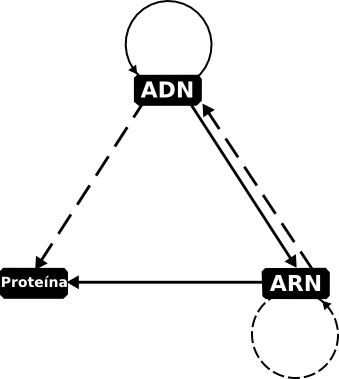
\includegraphics[scale=0.5]{./figures/dogma.jpg}
\caption{El dogma central de la biología molecular es un concepto que ilustra
la direccionalidad de los mecanismos y transmision de la información genética}
\end{figure}


\subsection{Niveles de organización de estudio bidireccional en la genética y  la Biología molecular}
\begin{figure}[htb!]
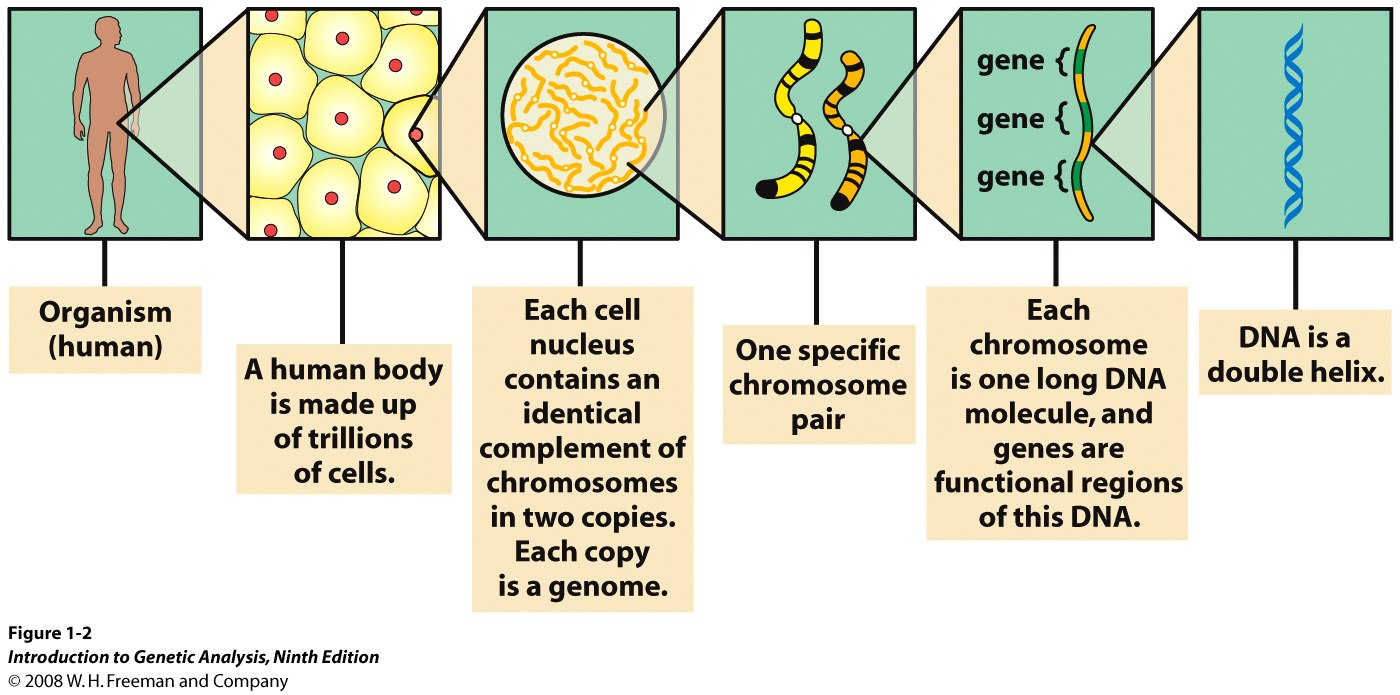
\includegraphics[scale=0.3]{./figures/figure02.jpg}
\caption{De nuestra vision general a la particular para el estudio de diferentes niveles de variación de variación. Los diferentes niveles de observacion nos muestran la escala de organizaci
on de componentes en cada nivel }
\end{figure}


\subsection{ Bases moleculares de la información genética}

Tres procesos principales en nuestras células aseguran la fidelidad del código y su correcta traducción y conservación. Estos tres procesos son la replicación del DNA, la transcripción y la 
traducción. 

\begin{figure}[htb!]
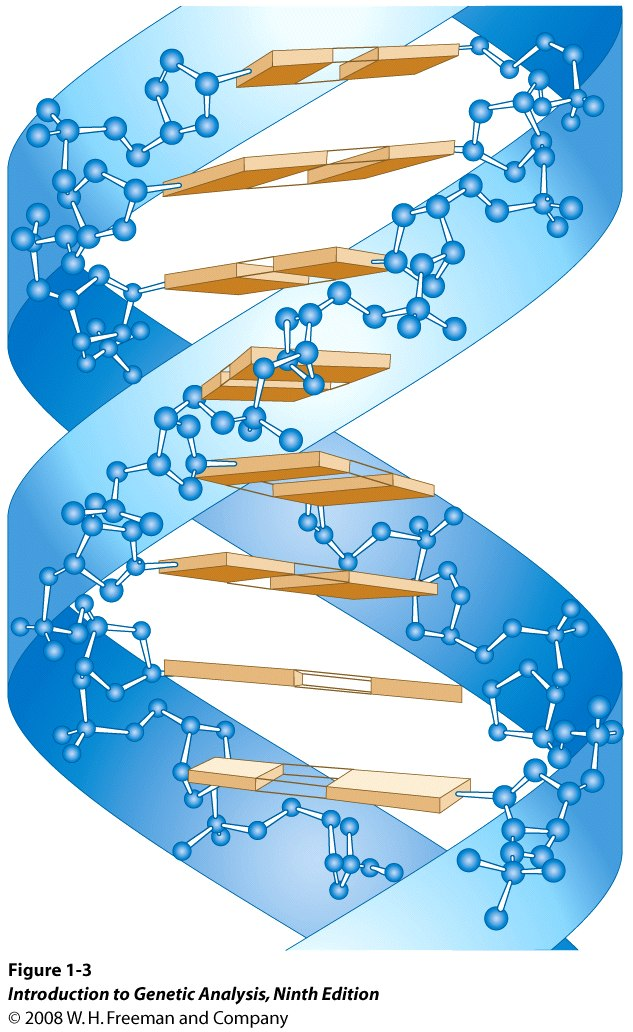
\includegraphics[scale=0.3]{./figures/figure03.jpg}
\caption{ Replicación: La estructura de los organismos y sus procesos fisiológicos se basan
en el funcionamiento de las proteínas. La información genética para la síntesis
de esas proteinas se almacena en el DNA. Una molecula de DNA es una helice
compuesta de dos cadenas que se unen por reglas de complementariedad A:T y
G:C}
\end{figure}


\begin{figure}[htb!]
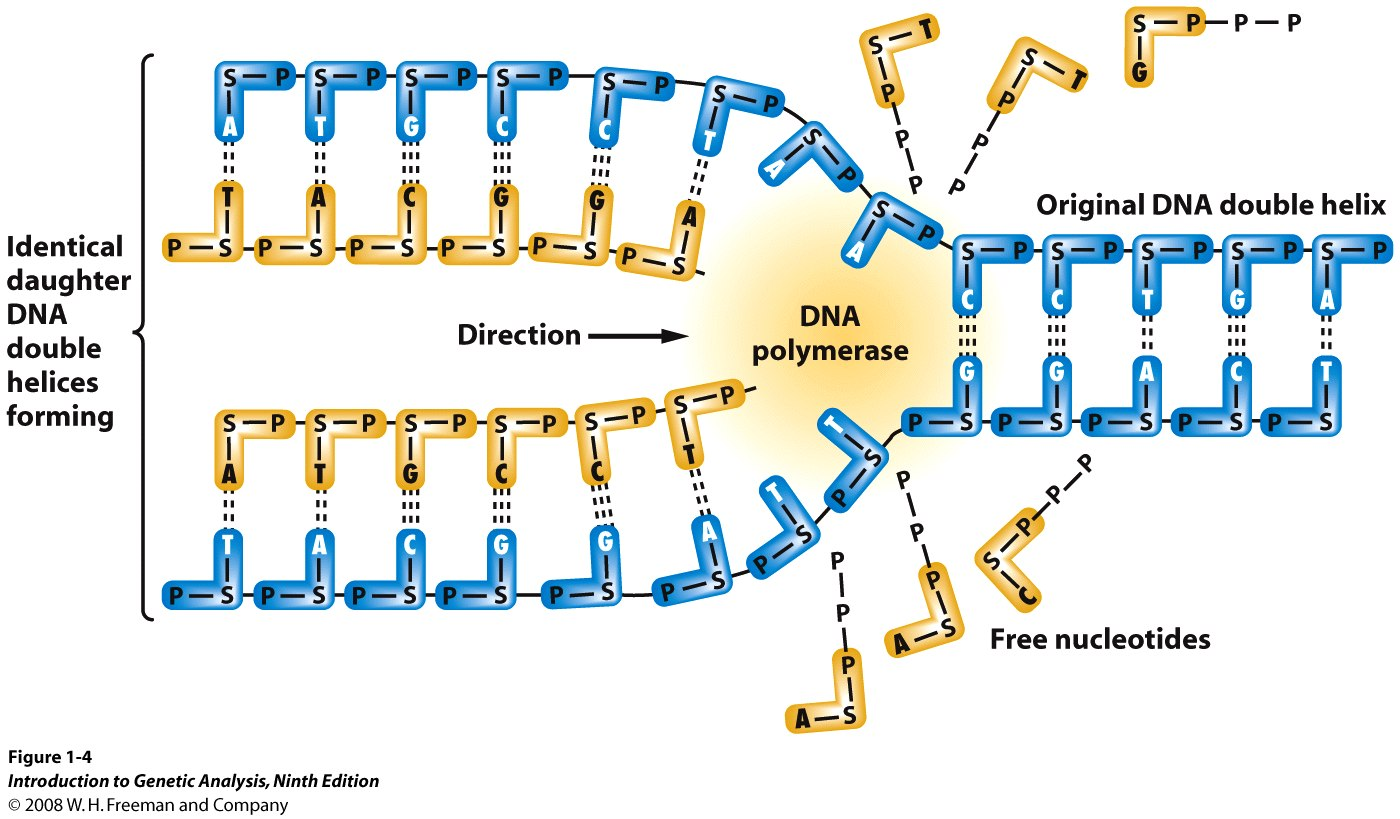
\includegraphics[scale=0.3]{./figures/figure04.jpg}
\caption{Replicación: En la replicacion del DNA nuevos nucleotidos son enlazados para formar
las cadenas hijas de DNA usando como molde las cadenas existentes. P (representa
fosfatos), S (Azucares) y A, C, G o T nucleotidos}

\end{figure}

\begin{figure}[htb!]
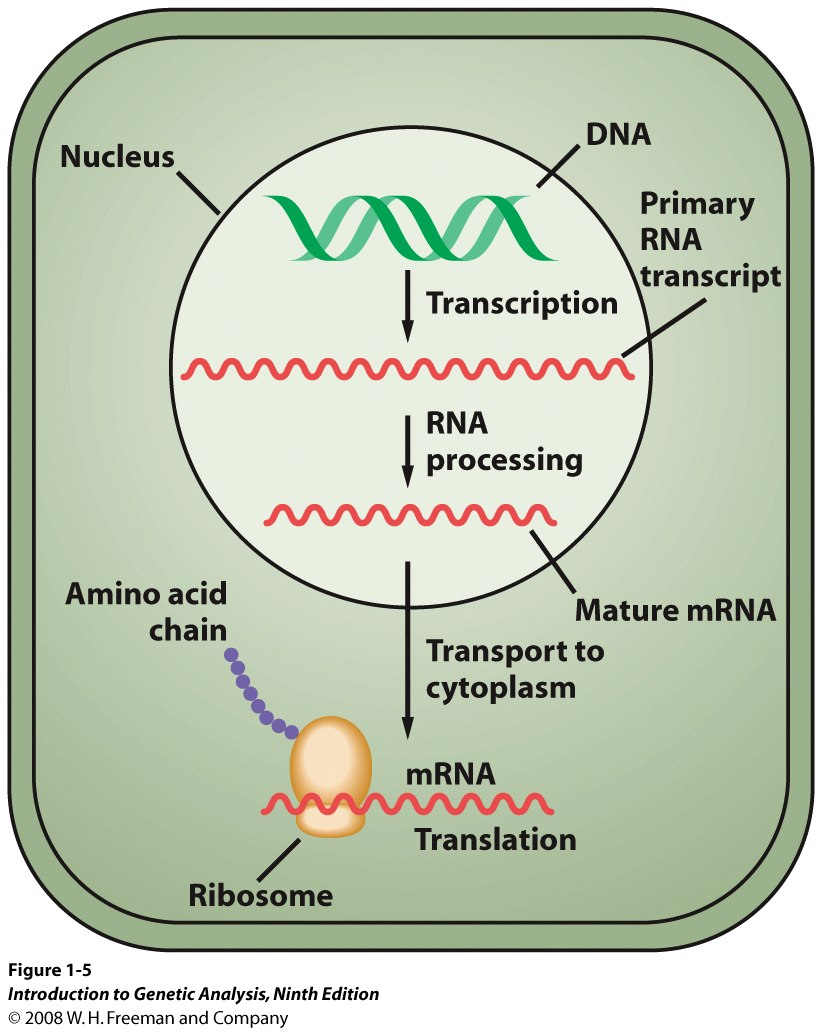
\includegraphics[scale=0.3]{./figures/figure05.jpg}
\caption{Transcripción:
En nuestras células el DNA se transcribe en RNA o RNA mensajero
y es transportado del nucleo de la célula al citoplasma donde ocurre la síntesis
de proteínas. Completando de esa manera el ciclo básico explicado en el dogma clásico de la biología molecular}
\end{figure}

\begin{figure}[htb!]
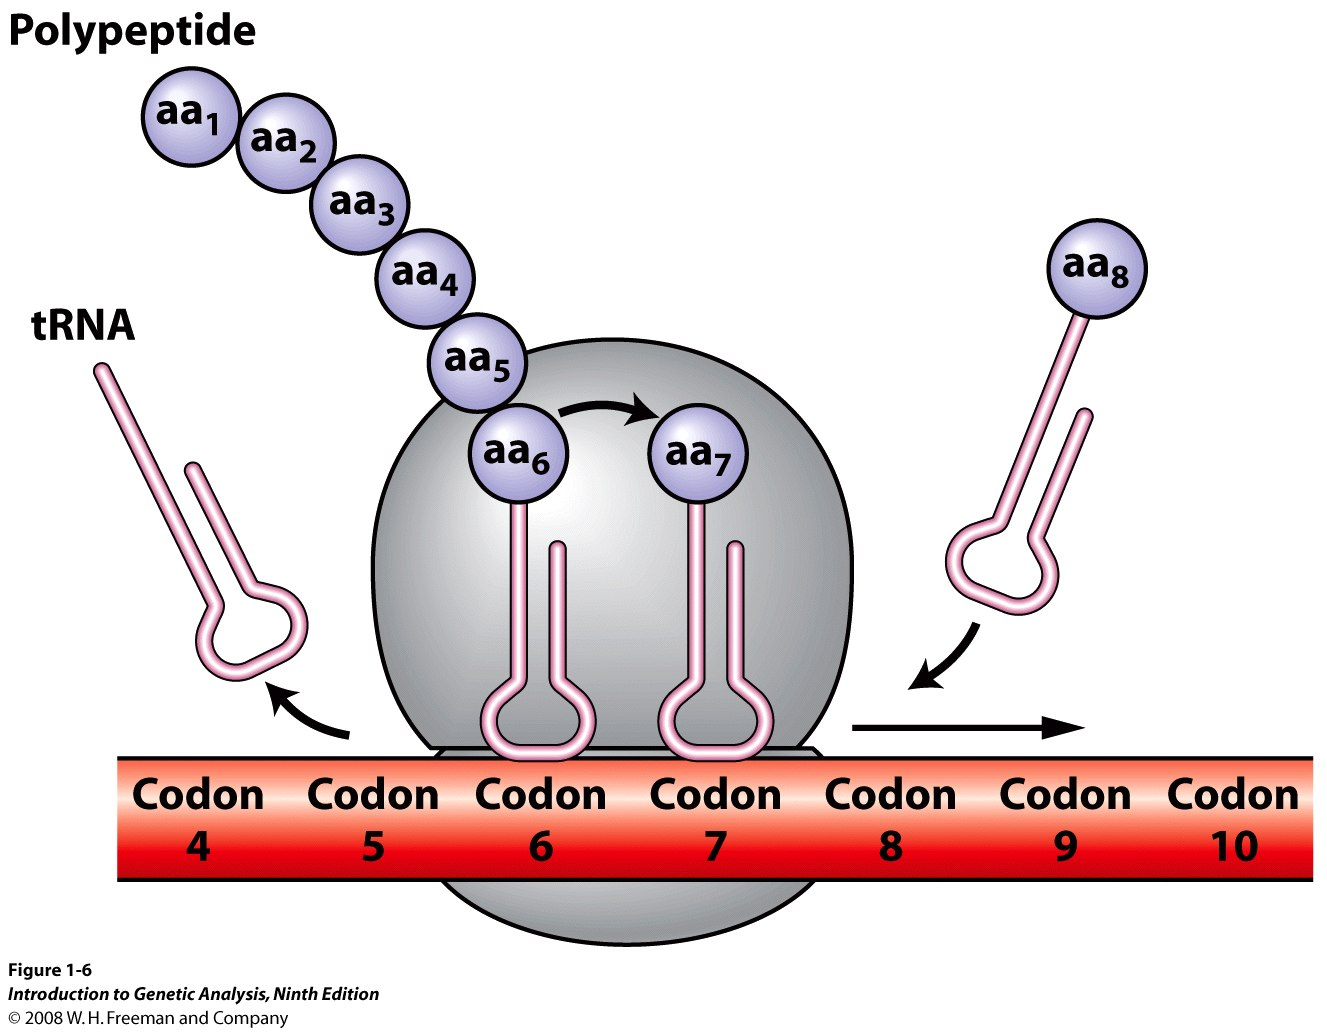
\includegraphics[scale=0.3]{./figures/figure06.jpg}
\caption{Traducción:
Un aminoácido se añade a la cadena naciente de proteíanas en el proceso
de traduccion de un mRNA y es en este proceso muy importante recordar el concepto de código genético}
\end{figure}


\newpage


\subsection{El código genético}
La primera idea importante de la biologia molecular es que el DNA es un libro
y como todo libro se debe leerse para tener sentido. No olvide consultar
http://www.intramed.net/contenidover.asp?contenidoID=42002 o \newline
http://www.nature.com/scitable/topicpage/dna-transcription-426 para ampliar
sus conceptos. Es importante recordar que la secuencia del DNA se compone
de 4 caracteres que representan los nucleotidos (A, G, C y T), y la secuencia
de RNA por otros 4 caracteres (A, G, C y U) que representan ribonucleotidos.
Por otro lado, las secuencias de proteinas se representan por otros 20 diferentes
caracteres (A,C,D, ... etc) que representan los 20 aminoacidos. El DNA se
transcribe a otro tipo de molécula el RNA por un proceso conocido
como transcripción (escribir con un sistema de caracteres lo que está escrito
en otro, es un concepto general que se acuña detrás de un código). En el paso final el mRNA es traducido por medio de la asignacion
de grupo de 3 ribonucleotidos (triplete) a un aminoacido.  El código genético
representa la regla para convertir una pieza de informacion (un triplete) en otra
forma o representacion (un aminoacido).


\begin{figure}[htb!]
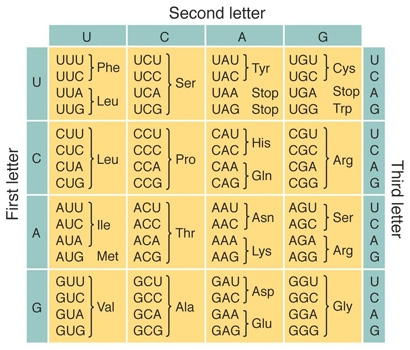
\includegraphics[scale=0.4]{./figures/codigo.jpg}
\caption{
Existe un orden para asignar cada nucleótido en el código, la primera y la segunda son siempre determinantes del tipo de aminoácido correspondiente y la tercera es menos importante en algunos casos}

\end{figure}



\end{document}
